\section{Practical Middleware for Massively Multiplayer Online Games}
The first architecture and it's design choices we are going to review, is the architecture described in \emph{Practical Middleware for Massively Multiplayer Online Games} \cite{middleware}.
In this paper the authors elaborated on the middleware platform. The purpose of such a platform is, how the authors stated it, "Middleware helps programmers manage the complexity and heterogeneity of distributed computing environments". So for short it is a platform which makes it easier to develop and maintain distributed games. The authors have also developed their own platform and have made several architectural design decisions for that. The platform is called Distributed organized Information Terra (DoIT) middleware platform. \\

\begin{wrapfigure}{r}{0.5\textwidth}
\begin{center}
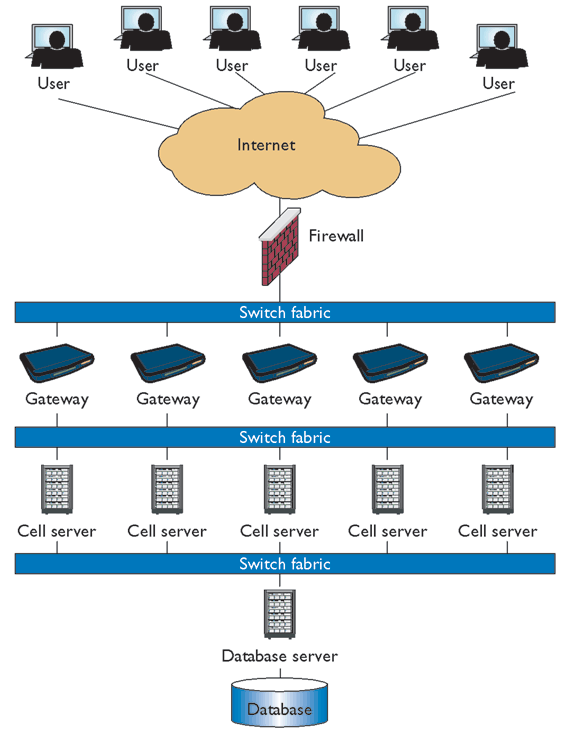
\includegraphics[width=0.4\textwidth]{4tier}
\caption{General framework for middleware platforms for MMOG}
\end{center}
\label{fig:4tier}
\end{wrapfigure}

\noindent A lot of research has been done by researchers to define a framework for middleware platforms. The framework is a 4-tier architecture consisting of a client, a proxy/gateway, a cell server and a database tier. The gamers have control over the client applications. The proxy is in charge of distribution of messages and security aspects. The cell servers maintain the virtual world, it also makes sure that no collisions appear between multiple game clients. The database stores the players states, so that all the changes people made are not wiped clean every time they log off. A graphical view of this architecture is shown in \autoref{fig:4tier} \cite{midfig}. \\
\indent Next to this general framework for the architecture there is also a list of properties which a a middleware platform should adhere to. These properties are \emph{Ease of Development}, \emph{Ease of Deployment}, \emph{Ease of Maintenance}, \emph{Ease of Change} and \emph{Performance and Load Balancing}. For an elaborated description of these properties, we refer to section "Practical Next-Generation MMOG Middleware" in \cite{middleware}.\\

\noindent Now we know the basics of a middleware platform, we shall discuss the architecture of the DoIT platform. This platform uses a message-oriented middleware instead of a RPC-based technology. The authors claim that this of great benefit due to the event-driven behavior of MMOG's. This seems logical. A lot of the game play of MMOG is indeed based on events made by other players. RCP does not really benefit from this, it would be better suited for single player games, because in that case all the procedure calls are done by the one client. \\
\indent Another great advantage of MOM over RCP is that MOM allows decoupling while RCP does not. This is also mentioned by the authors. Next to this difference the DoIT platform differs on two points from the framework mentioned before. The first is that DoIT is customizable and reduces the complexity for MMOG application programmers. The only proof for this, given by the authors, is that a code-generator model is introduced. This model generates message-factory and handler classes for a protocol. The developer still has to define the real detailed content for these handlers. We think that this seems not really enough evidence that this platform really reduces complexity for programmers. It only generates some code automatically (the handlers). The protocol still has to be defined by the programmer and the actual code in the handlers still has to be produced by the programmers. So in practical, the authors only stated that they made a module which generates the handlers for a protocol, but they still have to filled. The only real benefit from this is that you do not forget to create such a handler. So we think this claim is really questionable.\\
\indent The authors also made a small notion of security of their platform. The protocols are modeled as a set of message fields and the generator engine randomly shuffles these fields. This makes hacking specific messages more complicated. The authors also claim with just that this is not really safe yet and that messaging protocols and encryption algorithms are needed to prevent attacks.\\
\indent The last feature DoIT includes is a real-time virtual-world logic, called VWLogic. This logic has as a target to decrease the complexity for the programmers. The idea behind it is really nice. There is a VWLogic adapter which demultiplexes for each VWLogic component, as stated by the authors. When a message comes in, the VWLogic adapter finds the corresponding handler. After that handler is finished the VWLogic adapter sends an update request. Unfortunately the authors do not mention what architecture is used to accomplish this or give any proof of how this works. So the idea is really nice and the programmers certainly benefit from this, if it works.\\

\noindent Another question that comes to mind for these kind of platforms is, how does this architecture affects the game state of a client? This can all be derived from the general framework for middleware which DoIT follows. The MMOG has a central (or multiple, you can play with that a bit) database servers. In these servers the game state of a client is saved. This has as a great advantage that a client user does not depend on the availability of other users (like in a P2P network). The downside of this is that a lot of traffic has to go from/to that database server. \\
The framework tries to minimize this by letting several cell servers interact with this database server. Fortunately this database server does not have to be interacted very often, I assume once to load the clients game state when he logs on and once to store it when he logs of. The massive interaction happens between clients and cell servers. Now I assume that all one cell server handles the game server in which clients are playing or that when several cell servers handle such a game server that they communicate with each other. Otherwise it would not be possible to resolve conflicts between clients, like for instance user A picks up an item and user B picks up the same item at about the same time. This conflict has to be resolved by the client servers. Luckily this can be easily done by doing a request to the server whether this item can be picked up or not. The cell server(s) only allow one of those request. So this client server architecture in the 4-tiered framework ensures that client games are in a steady state.\\
There is now one problem that have to be addressed, that is what happens when one of the cell servers or database servers goes down? When one of the cell servers goes down, than it is possible to distribute the clients over other cell servers. This might affect the performance a bit, due to bigger loads on the other cell servers but it is still better than just dump the connections with the clients that were connected to the failed cell server. A bigger issue is what happens when the database server goes down? Do they have backup servers for that? As shown in the architecture in \cite{midfig} there is only one database server. So when this server is down, the game cannot be played. However we assume that there are (several) backup servers for this database server. In that way the game can still be played.


